\capitulo{5}{Aspectos relevantes del desarrollo del proyecto}

El inicio de este proyecto comenzó el septiembre, pero he creído conveniente rehacerlo de cero varias veces para mejorar ciertos aspectos desde el principio, darle un nuevo enfoque y no arrastrar errores iniciales. Por ello en este apartado voy a hablar sobre los aspectos relevantes de las dos partes principales del proyecto: \textit{Raspberry Pi} y \textit{Aplicación Android}.

\section{Raspberry Pi}

En cuanto a esta parte vamos a diferencias tres partes importantes del proyecto: \textit{Interfaz}, \textit{Servidor Python} y \textit{Base de datos}.

\subsubsection{Interfaz}

La interfaz en la Raspberry Pi 3 está desarrollada mediante la librería \textit{Tkinter}. Esta librería viene incorporada con Python 3 y es bastante sencilla de utilizar, pero el problema que tiene con respecto a otras tecnologías, es que sus elementos y posibilidades son limitados. Pero tras investigar, encontré que a partir de la versión 8.5 de \textit{Tkinter} se introdujo un módulo llamado \textbf{ttk} que nos permite un nuevo abanico de posibilidades. Entre dichas posibilidades encontramos widgets como \textit{ComboBox}, \textit{Notebook}, \textit{Progressbar}, etc. 

Leyendo sobre su utilización, comencé a trabajar con un ComboBox rellenándolo con las estancias y teniendo la posibilidad de eliminar la estancia seleccionada en él. Una vez avanzado el proyecto, y tras cambiar los objetivos para que el servidor no tuviese la capacidad de realizar cambios de manera independiente a la aplicación, me metí con la \textit{Notebook}. Esta ha sido la mejor manera de representar nuestra casa, de manera que cada \textit{pestaña} o \textit{tab} será cada una de las estancias, y dentro del contenido de cada \textit{pestaña} se representa la iluminación. Su creación, modificación y eliminación es bastante sencilla, el único problema se encuentra en la inserción de objetos en el contenido de la pestaña. El problema es que el contenido de la pestaña y la pestaña son cosas diferentes. El contenido de la pestaña es un \textit{Frame} que se acopla a la pestaña en su creación, de tal manera que cuando tratamos de insertar elementos en ella no necesitamos referenciar a la pestaña, sino al \textit{Frame}. Por ello, me ví obligado a mantener una estructura que contiene todos los \textit{Frames} de las pestañas activas, de tal manera que se van añadiendo y eliminando según lo vayando haciendo las pestañas correspondientes.

Un problema similar me surgió para conseguir poder modificar las \textit{labels} o \textit{etiquetas} que representan las bombillas. Estas \textit{etiquetas} están representadas dentro de dichos \textit{Frames}, pero no son accesibles a través de él. Por tanto, me ví de nuevo obligado a crear y mantener una nueva estructura que contiene todas las \textit{etiquetas} o bombillas que tenemos actualmente. Esta segunda estructura es diferente de la primera, ya que la primera era una simple lista y esta es un tabla \textit{hash}. En esta estructura la clave será el nombre de la pestaña, es decir, el de la estancia y el valor, será una lista con los identificadores de las etiquetas de esa pestaña para poder acceder a ellas.

Y por último, hay que tener en cuenta que para la representación de la interfaz, el objeto que la crea se mantiene mediante un bucle infinito. Por tanto, no se deberían realizar inicializaciones ni cambios dentro del código de dicho bucle. Respecto a la interfaz estos son los aspectos más relevantes ya que se intentó simplificar lo más posible su complejidad.

\subsection{Servidor Python}

El servidor Python lo hice con la finalidad de que siempre estuviese escuchando los cambios que le llegan de la aplicación. Lo primero que me sucedió, es que no podía crearlo a la vez que la interfaz, debido a que la interfaz se encuentra en un bucle infinito. Debido a esto, se me ocurrió crearlo al inicio, pero en un \textit{Thread} o \textit{Hilo} independiente. 

La otra parte complicada del servidor, ha sido lo que llamo el tratamiento de datos. Por tratamiento de datos me refiero a la interpretación de los mensajes de los clientes de tal manera que produzcan cambios reales en nuestra interfaz. La interpretación de mensajes de realiza de la siguiente manera:

\begin{itemize}
	\item \textbf{Añadir estancia:} \textbf{+} (Añadir) \textbf{E} (Estancia) \textbf{nombre} (Nombre de la estancia) Ej.: +EHabitación 1
	\item \textbf{Añadir una bombilla:} \textbf{+} (Añadir) \textbf{B} (Bombilla) \textbf{número} (Posición de la estancia) \textbf{nombre} (Nombre) Ej.: +B2Bombilla1
	\item \textbf{Modificar estancia:} \textbf{*} (Modificar) \textbf{E} (Estancia) \textbf{número} (Posición de la estancia) \textbf{nombre} (Nombre al que queremos cambiar) Ej.: *E1Habitación 2
	\item \textbf{Modificar bombilla:} \textbf{*} (Modificar) \textbf{B} (Bombilla) \textbf{número} (Posición de la estancia) \textbf{número} (Posición de la bombilla) \textbf{nombre} (Nombre al que queremos cambiar) Ej.: *B02Bombilla Azul
	\item \textbf{Eliminar estancia:} \textbf{-} (Eliminar) \textbf{E} (Estancia) \textbf{número} (Posición de la estancia) Ej.: -E1
	\item \textbf{Eliminar bombilla:} \textbf{-} (Eliminar) \textbf{B} (Bombilla) \textbf{número} (Posición de la estancia) \textbf{número} (Posición de la bombilla) Ej.: -B12
	\item \textbf{Cambiar estado bombilla:} \textbf{\#} (Cambiar) \textbf{número} (Estado, 1: Encender 0: Apagar) \textbf{número} (Posición de la bombilla en la estancia) \textbf{nombre} (Nombre de la estancia) Ej.: \#11Habitación 1
	\item \textbf{Borrar base de datos:} \textbf{/} (Borrar la base de datos) Ej.: /
	\item \textbf{Mandar la base de datos actual al cliente:} \textbf{<} (Actualizar) Ej.: <
\end{itemize}

Para que la función de mandar la base datos al cliente funcione correctamente, mandando un mensaje por cada acción es necesario introducir un pequeño retardo entre mensaje y mensaje. Sino el cliente lo recibirá todo como un mensaje de gran longitud y no podrá tratarlo correctamente.

Al final del proyecto se decidió hacer el servidor fuese multiusuario y que varias personas a la vez pudiesen realizar cambios. Esto llevó algo de trabajo no solo en la parte del servidor, sino en la parte del cliente, que tiene que recibir los cambios, tratarlos en el momento y actualizar su vista.

\subsection{Base de datos}

La base de datos utilizada para mantener la persistencia de los elementos de nuestro hogar ha sido \textbf{Sqlite3}. Sqlite es un sistema de gestión de base de datos de pequeño tamaño que permite realizar operaciones básicas de manera muy sencilla. Entre las opciones de persistencia es la que más me ha gustado debido a su sencillez y funcionamiento.
Para mantener la persistencia he creado operaciones básicas como guardar, recuperar, modificar y actualizar valores de las tablas \textit{estancias}, \textit{elementos} y \textit{tableIp}. Podemos observar un ejemplo de cada tabla en las tablas \ref{tabla:tablaEstanciasPython}, \ref{tabla:tablaElementosPython} y \ref{tabla:tablaTableIpPython}.

\tablaSmall{Ejemplo de datos de la tabla \textit{estancias}.}{l c c c c}{tablaEstanciasPython}
{ \multicolumn{1}{l}{}id & nombre \\}{
	0 & Habitación 1\\
	1 & Salón 1\\
	2 & Cocina 1\\
	3 & Baño 1\\
}


\tablaSmall{Ejemplo de datos de la tabla \textit{elementos}.}{l c c c c}{tablaElementosPython}
{ \multicolumn{1}{l}{} estancia & nombre & estado \\}{
	Habitación 1 & Bombilla 1 & 0\\
	Habitación 1 & Bombilla 2 & 0\\
	Salón 1 & Bombilla 1 & 1\\
}

\tablaSmall{Ejemplo de datos de la tabla \textit{tableIp}.}{l c c c c}{tablaTableIpPython}
{ \multicolumn{1}{l}{} id & ip \\}{
	0 & 192.168.X.X\\
}

\section{Aplicación Android}

La aplicación Android ha sido la parte más complicada de este proyecto, ya que es más la extensa y compleja del proyecto. Por ello vamos a hablar de cierto puntos importantes.

\subsection{Persistencia}

La aplicación esta dividida en tres \textit{Activity} o ventanas diferentes. Uno de los problemas más importantes es sin duda la persistencia de los elementos cuando nos movemos entre ellas. Resulta que cada vez que abandonamos una y nos dirigimos a otra, la primera llama a su método \verb|onDestroy|, y cuando volvemos de la segunda a la primera llama a su método \verb|onCreate|. Esto es lo que se llama ciclo de vida de una \textit{Activity} \ref{fig:cicloDeVida}. Cuando una ventana no está en la vista actual se destruye y cuando se vuelve a ella se crea de nuevo. El problema está en que nosotros manejamos los elementos dinámicamente, es decir, el método \verb|onCreate| solo nos crea la ventana vacía como la primera vez que abrimos la aplicación, y somos nosotros los que manualmente añadimos más elementos a esa vista. Entonces, cada vez que nos desplazamos entre ventanas, se está llamando al método \verb|onCreate| y nos representa dicha ventana vacía y perdemos los elementos creados dinámicamente.

\begin{figure}[h!]
	\centering
	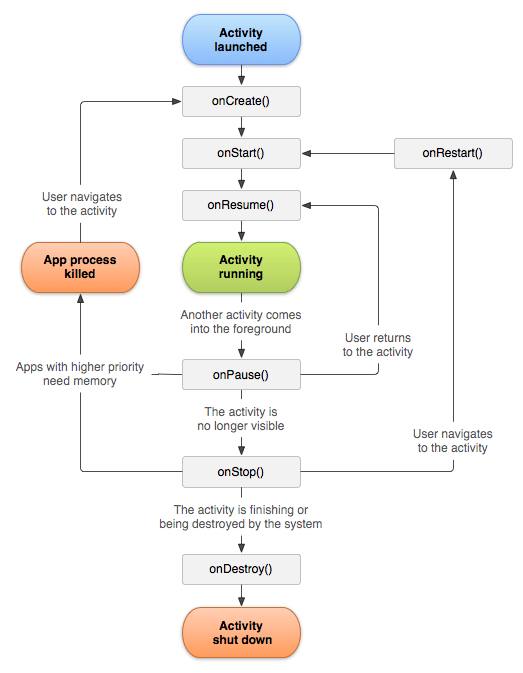
\includegraphics[width=1\linewidth]{img/cicloDeVida}
	\caption{Ciclo de vida de una \textit{Activity} en Android.}
	\label{fig:cicloDeVida}
\end{figure}

Para evitar este problema es necesario crear una forma de mantener la persistencia de los elementos. Por ello, opté por crear una base de datos en \textbf{Sqlite} como en la parte de Python. Y dentro del método \verb|onCreate| de cada ventana que lo necesite, haremos una llamada a la base de datos para obtener los elementos que teníamos antes.

En la base de datos creada para Android tenemos las tablas \textit{estancias}, \textit{elementos} y \textit{datosServidor}. Podemos observar un ejemplo de cada tabla en las tablas \ref{tabla:tablaEstancias}, \ref{tabla:tablaElementos} y \ref{tabla:tablaDatosServidor}.

\newpage
\tablaSmall{Ejemplo de datos de la tabla \textit{estancias}.}{l c c c c}{tablaEstancias}
{ \multicolumn{1}{l}{}id & nombre \\}{
	0 & Habitación 1\\
	1 & Salón 1\\
	2 & Cocina 1\\
	3 & Baño 1\\
}

\tablaSmall{Ejemplo de datos de la tabla \textit{elementos}.}{l c c c c}{tablaElementos}
{ \multicolumn{1}{l}{} estancia & nombre & estado \\}{
	Habitación 1 & Bombilla 1 & 0\\
	Habitación 1 & Bombilla 2 & 0\\
	Salón 1 & Bombilla 1 & 1\\
}

\tablaSmall{Ejemplo de datos de la tabla \textit{datosServidor}.}{l c c c c}{tablaDatosServidor}
{ \multicolumn{1}{l}{} id & ip & puerto\\}{
	0 & 192.168.X.X & 8888\\
}

\subsection{Visualización}

En este apartado visualización quiero hacer referencia a la forma de representación de las estancias y bombillas en la aplicación.

Para su correcta representación estaba buscando un método o estructura que me permitiese almacenar, modificar y eliminar de manera sencilla. Entonces se me ocurrió utilizar una \textit{ListView}, es decir, una lista de elementos. Esta estructura tiene sus propios métodos para realizar la agregación, eliminación y modificación, pero yo pretendía tener una \textit{ListView} personalizada. Pretendía que dentro de cada elemento o fila de la \textit{ListView}, se pudiese insertar más elementos como imágenes, botones, interruptores, etc. Debido a esto, no me quedó otra opción que crear una \textit{ListView} personalizada para las estancias y otra totalmente diferente para las bombillas. \\
Los elementos de la \textit{ListView} son organizados y tratados mediante un adaptador, que es el que representa los elementos en la lista. Por tanto, creé dos clases nuevas que heredasen de la clase \textit{ArrayAdapter} y así personalizarlas con mis preferencias. Una vez creadas, simplemente se crea una \textit{ListView} y se asigna un nuevo adaptador: 

\verb|listView.setAdapter(adaptador);|

Tras conseguir la estructura personalizada y que los elementos se viesen como quería, necesitaba alguna manera de que el usuario modificase los elementos de forma sencilla. Entonces se me ocurrió crear un menú contextual sobre cada elemento de la lista que permite realizar modificaciones solo sobre ese. Para conseguir que el menú contextual funcione sobre una \textit{ListView} hay que tener en cuenta que en la vista o \textit{layout} de la fila, esté activada la opción que permita mantener pulsado un largo tiempo. Es decir, necesitamos acceder a nuestro adaptador personalizado y añadir lo siguiente:

\verb|row.setLongClickable(true);|

Existe otro problema respecto a las \textit{ListView} y es que hay que tener en cuenta que los cambios realizados sobre la vista de cada elemento de la lista no van a permanecer una vez se llame a \verb|NotifyDataSetChanged()|. Este método lo que hace es cargar de nuevo los elementos de donde esta obteniendo la \textit{ListView} los datos. Por tanto, para conseguir añadir nuevos elementos y que tras llamar a este método, no desaparezcan los cambios realizados, en vez de realizar los cambios sobre la vista, tenemos que realizarlos sobre la lista desde la que toma los elementos la \textit{ListView}.

\subsection{Conexión}

Esta es la parte más importante de la aplicación Android y con la que más problemas me he encontrado.
Cuando comencé, la manera que me pareció más correcta para enviar datos al servidor era a través de un tarea asíncrona, es decir, es una ejecución independiente de la parte gráfica que estamos viendo. Dentro de ella, abría una conexión mediante un \textit{Socket}, enviaba el mensaje y lo cerraba de nuevo. 

Pronto me dí cuenta de que de esta manera yo no podría recibir mensajes del servidor en cualquier momento y me interesaba. Así que opté por hacer como en la parte del Servidor Python, crear una ejecución independiente mediante un \textbf{Thread} y escuchar siempre si llega algún mensaje del servidor.\\
Para conseguir que la ejecución de escucha del servidor funcionase tuve que crear una nueva clase que implementase la interfaz \textit{Runnable} y de está manera meter mi código en el método \verb|run()|. Además, una ventaja que tiene ser una ejecución independiente, es que no se interrumpe a pesar de realizar cambios entre ventanas. Yo quería que el mensaje que llegase fuese mostrado en pantalla y no es posible mostrar un mensaje en pantalla desde una ejecución independiente que no tiene parte gráfica.\\
Estuve indagando sobre como poder mandar mensajes, incluso objetos, desde un \textbf{Thread} a la parte gráfica y me encontré con la clase \textit{Handler} \cite{android:Handler}. La clase \textit{Handler} permite enviar y procesar mensajes y objetos asociados a la cola de un hilo. Entonces me di cuenta de que la manera de poder transportar el dato \textit{String} obtenido del servidor es encapsulado a través de un objeto \textit{Bundle}.

El método \verb|sendMessage| nos permite poner en la cola un objeto \textit{Message} que contendrá nuestro \textit{Bundle} con nuestros \textit{String} recibido. Una vez nuestro \textit{Bundle} llegue, será procesado por el método \verb|handleMessage|. Entonces lo ideal es sobreescribir ese método en una de las \textit{Activity} para poder realizar los cambios pertinentes sobre el dato recibido.

A la hora de la creación del \textit{Socket}, es mejor optar por crear un \textit{Socket} sin conexión mediante el constructor vacío y luego conectarlo, que intentar instanciar un \textit{Socket} con una ip y un puerto al inicio.\\
Otro problema respecto a la escucha del servidor es que cada vez que se trataba de conectar a través de la ventana del Servidor se creaba un nuevo hilo y esto daba lugar a que pudiésemos tener más de 5 hilos activos a la vez. Para solucionar este problema traté de usar un patrón de diseño \textit{Singleton}, que haría que solamente hubiese una única conexión y fuese accesible desde cualquier punto de la aplicación. De esta manera podemos realizar la conexión al servidor según entremos a la aplicación desde la ventana principal.
No he seguido el patrón de diseño al pie de la letra ya que en él se especifica que el objeto no tiene parámetros, pero el mío si los tiene. Y esto sucede porque a la hora de implementar la posibilidad de ser más usuarios conectados al servidor, necesitaba una manera de saber en que ventana nos encontramos para actualizar sus elementos según el mensaje que llegue.\\
Además este patrón de diseño ha sido usado debido a que para cerrar la conexión activa con el servidor, necesitamos acceder a la instancia de \textit{RecepcionSocket} que se usó para la creación del hilo. Es decir, de está manera, la conexión que se crea en la ventana principal es posible cerrarla desde la ventana del Servidor, ya que estamos accediendo a la misma instancia \textit{RecepcionSocket} que se usó en la creación.

Por último, quería decir que he tenido muchos problemas a la hora de saber si la conexión ha llegado a conectarse, está activa o cerrada. Es decir, si yo quisiese saber si ahora mismo estamos conectados al servidor, no he encontrado una manera sencilla de averiguarlo. El problema es que los métodos de los que nos provee la clase \textit{Socket} no son nada claros.

\begin{itemize}
	\item El método \verb|isConnected()| \cite{android:isConnected} de la clase \textit{Socket} indica que cerrar un \textit{socket} no borra su estado de conexión, lo que significa que este método devolverá un \textbf{True} aunque el \textit{socket} esté cerrado si se ha llegado a conectar alguna vez.
	\item El método \verb|close()| \cite{android:close} de la clase \textit{Socket} indica que una vez se ha cerrado el \textit{socket} no estará disponible para nuevas conexiones, es decir, no puede ser reconectado. Por tanto, es necesario crear una nueva instancia del \textit{Socket}.
\end{itemize}

Esto hace que haya muchos problemas para saber si tenemos una conexión activa con el servidor.
